Als erster Kandidat wurden Lipide untersucht, da diese schon in Vorarbeiten benutzt wurden, um dünne Eisschichten mittels Plungefreezing zu erhalten.

\section{Lipide}

Die Löslichkeit der Lipide bei Raumtemperatur wurden bei sieben verschiedenen Lösungsmitteln getestet. Für diesen Versuch wurden Glasträger zuerst mit Lipiden benetzt, dafür wurde diese in vorgefertigte Lipidlösung eingetaucht und angetrocknet. Dann wurde ein Vergleichsbild von den Schlieren der abgelagerten Lipiden unter dem Mikroskop aufgenommen. Anschließend wurden die benetzten Glasproben in ein Behälter mit dem Lösungsmittel gegeben und für eine kurze Zeit (unter 15 min) gewartet. Danach wurde die Glasprobe wieder herausgeholt und unter einen Mikroskop verglichen. Keine Veränderung der Schlieren weist auf keine Lösbarkeit hin, Veränderungen und teilweise verschwinden der Schlieren deutet auf eine teilweise Lösbarkeit hin und eine saubere Glasoberfläche zeigt eine vollständige Lösbarkeit der Lipide.

\begin{table}[h]
	\centering
	\begin{tabular}{|l|c|c|}
		\hline
		Lösungsmittel & Lösbarkeit EGG-PC & Lösbarkeit DOPC \\
		\hline
		\hline
		4-Methyl Pentene & vollständig & N/A  \\ 
		\hline
		3-Methyl Pentene & teilweise & keine \\
		\hline
		1-Pentene & keine & keine \\
		\hline
		Isopentane & keine & teilweise\\
		\hline
		1-Propanol & vollständig & vollständig\\
		\hline
		Pentane & vollständig & keine\\
		\hline
		Ethanol & N/A & vollständig\\
		\hline
	\end{tabular}
	\caption{Getestete Lipide und Lösungsmittel unter Raumtemperaturen}
	\label{table:LoeslichkeitRaumtemperatur}
\end{table}

Aus diesen Versuchen geht hervor, dass jeweils drei verschiedene Lösungsmittel EGG-PC bzw. DOPC vollständig lösen können (Tabelle \ref{table:LoeslichkeitRaumtemperatur}). Im Anschluss wurden diese Lösungsmittel bei einer Temperatur von -140°C ebenfalls auf Löslichkeit untersucht. Da nicht alle dieser Lösungsmittel sind flüssig bei -140°C sind, wurden diese entweder bei höheren Temperaturen untersucht oder mit anderen Stoffen oder Lösungsmitteln mit niedriger Schmelztemperaturen vermischt, als versuch die Schmelztemperatur des gesamten Gemisch zu reduzieren \ref{table:SchmelztemperaturLösungsmittel}. Jedoch lassen sich manche Lösungsmittel nicht vermischen, wodurch keine Schmelztemperaturverringerung erzielt werden konnte. 

Der Versuch zeigt, dass manche Lösungsmittel EGG-PC und DOPC lösen konnten, aber keine vollständiges Lösen der Lipide auf dem Glasobjektträger erreichten\ref{table:Cryoloeslichkeit}. Da für eine Anwendung zum Ablösen der Eisschicht eine sehr gute Lösbarkeit bei Cryotemperaturen vorrausgesetzt sind, wurden andere Verfahren als Vielversprechender bewertet. 

\begin{table}[h]
	\centering
	\begin{tabular}{|c|c|}
		\hline
		Lösungsmittel & Schmelztemperatur in °C \\
		\hline
		\hline
		4-Methyl Pentene & -154 \\ 
		\hline
		3-Methyl Pentene & -154 \\
		\hline
		1-Pentene & -165 \\
		\hline
		Isopentane & -160 \\
		\hline
		1-Propanol & -126 \\
		\hline
		Pentane & -129 \\
		\hline
		Ethanol & -114 \\
		\hline
	\end{tabular}
	\caption{Schmelztemperaturen in °C für verschiedene Lösungsmittel.}
	\label{table:SchmelztemperaturLösungsmittel}
\end{table}

\begin{table}[h]
	\begin{subtable}{\linewidth}
		\centering
		\begin{tabular}{|c|c|}
		\hline
		Lösungsmittel & Lösbarkeit \\
		\hline
		Pentane & 3h bei -125°C \\
		\hline
		4-methyl pentene & Nicht lösbar \\
		\hline
		\makecell{1:1 Volumenverhältnis\\ HFE zu 1-Propanol} & \makecell{Nicht gemischt,\\ 1-Propanol gefroren,\\ nicht ausreichende lösbarkeit}\\
		\hline
		Flüssiges Ethan & Nicht lösbar \\
		\hline
		\end{tabular}
		\caption{EGG-PC}
		\label{table:EGG-PCCryoloeslichkeit}
	\end{subtable}
	\begin{subtable}{\linewidth}
		\centering
		\begin{tabular}{|c|c|}
		\hline
		Lösungsmittel & Lösbarkeit \\
		\hline
		\makecell{1:4 volumenverhältnis\\ bzw. 1:2 molares verhältnis\\ Ethanol zu Isopentane} & 15 min geringe löslichkeit\\
		\hline
		\makecell{1:2 volumenverhältnis\\ bzw. 1:1 molares verhältnis\\ 1-Propanol zu Isopentane} & Nicht lösbar \\
		\hline
		Isopentan & 15 min geringe löslichkeit\\
		\hline
		1-Propanol & \makecell{15 min bei -130°C\\ geringe löslichkeit beobachtet}\\
		\hline
		Flüssiges Ethan & Nicht lösbar \\
		\hline
		\end{tabular}
		\caption{DOPC}
		\label{table:DOPCCryoloeslichkeit}
	\end{subtable}
	\label{table:Cryoloeslichkeit}
\end{table}

\section{Finger}

Für alle folgenden Versuche wurden ebenfalls Glasobjektträger eingesetzt, welche mit EGG-PC Beschichtet wurden. Anschließend wurde eine dünne Eisschicht mit beigemischten Fluoreszin ??mg/50ml auf dem Objektträger eingefrohren.

\subsection{Kleberdosierung}

INSERT FIGURE MIT 4.10 BIS 4.50 HERE VIELLEICHT RAUS AUS DEM ERGEBNISTEIL
	
\subsection{Temperaturtest}

QUANTIFIZIEREN ANSTATT NUR SAGEN ES WIRD HÄRTER????

\subsection{Ablöserichtung}

NO DATA HERE TOO

\subsection{Ablöseversuche Plunge gefreezte proben}

Ein weiterer Faktor, welche die Ablösbarkeit der Eisschicht beeinflussen könnte, ist die Dicke der Eisschicht. Im folgenden wurden Proben, welche mit einen Plungefreezer eingefroren sind, getestet. Es wurde anschließend verglichen, bei wie vielen Proben erfolgreich ein Teil der eisschicht abgelöst wurden im Vergleich zu vorherigen versuchen. Es lässt sich erkennen, dass durch die Dicke der Eisschicht kein leichteres Ablöseverhalten zu erkennen ist.

\begin{table}
	\centering
	\begin{tabular}{|c|c|c|}
		\hline
		Einordnung einzelner Versuche& Hand eingefroren & Plungefreezer \\
		\hline
		\hline
		Komplett durchgeführte Versuche & 4 & 4\\
		\hline
		Nicht erfolgreich & 3 & 3\\
		\hline
		Brüche/klare Bewegung & 1 & 1\\
		\hline
		Stück am Finger & 0 & 0\\
		\hline		
	\end{tabular}
	\caption{Vergleich der Ablösbarkeit von Hand eingefrorene Proben und Proben eingefrorene Proben}
\end{table}

\section{PDMS}

Nun werden zwei Mischungsverhältnisse von PDMS gegeneinander verglichen. Dazu wurden jeweils Proben erstellt mit jeweils 4:1 und 1:2 Base coat zu curing agent Mischungsverhältnis. Diese wurden mithilfe der Zugmaschine untersucht. Dafür wurde ein Stempel aus Plexiglas mit UV-Kleber an die Schicht geklebt und anschließend mit konstanten wegänderung in NAMEN DER RICHTUNG VERGESSEN abgezogen. Dies wurde mehrere Male wiederholt. Das Ergebnis zeigt, dass das Mischungsverhältnis 4:1 generell mit mehr Zugspannung abgerissen wird als 1:2 (Abb.\ref{fig:vgl4:1zu1:2zuGlas}). Auch die Literatur weist darauf hin, dass Eis generell schlechter auf 1:2 Mischungsverhältnis haftet als auf 4:1\cite{IbanezIbanez.2022}. Deswegen wurde im Folgenden das Mischungsverhältnis 1:2 gewählt, da diese bessere Grundeigenschaften zum Ablösen einer Eisschicht liefern, egal bei welcher Trennschicht sich das Eis von dem Objektträger lösen wird.


\begin{figure}
	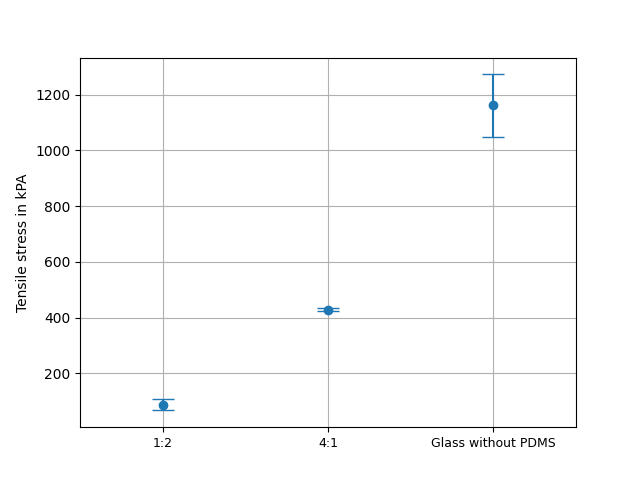
\includegraphics[width=14cm]{plotVGLZugspannungPDMSMischungsverhaeltnisse}
	\caption{Vergleich 4:1 zu 1:2 Base coat zu curing Agent und Glas ohne PDMS}
	\label{fig:vgl4:1zu1:2zuGlas}
\end{figure}


Anschließend wird der Effekt von Plasmacuring auf PDMS untersucht. Dafür wurde der gleiche Aufbau mit der Zugmaschine verwendet. Die Probe wurde möglichst kurzzeitig nach der Plasmaaktivierung in die Zugmaschine Eingespannt und verklebt. Auch mit den geringen Wiederholungsraten ist ein deutlicher Anstieg der Zugspannung über zunehmender Plasmaaktivierung zu sehen (Abb. \ref{fig:PlotPlasmaAktivierung}). Bei Längerer Aktivierung wird die Zugspannung teilweise versechsfacht. Da die wiederholungsraten sehr klein sind, kann hier gut eine Tendenz gezeigt werden, aber keine genaue aussagen wie hoch die Kraft bei gegebener Plasmaaktivierung ist. Ebenfalls ist das Ergebnis nicht übertragbar auf andere Mischunsverhältnisse, da diese andere Eigenschaften haben, welche zu einen glass-like zustand durch Plasmaaktivierung erreichen können QUELLE. Dieser wurde hier nicht beobachtet. 


\begin{figure}[h]
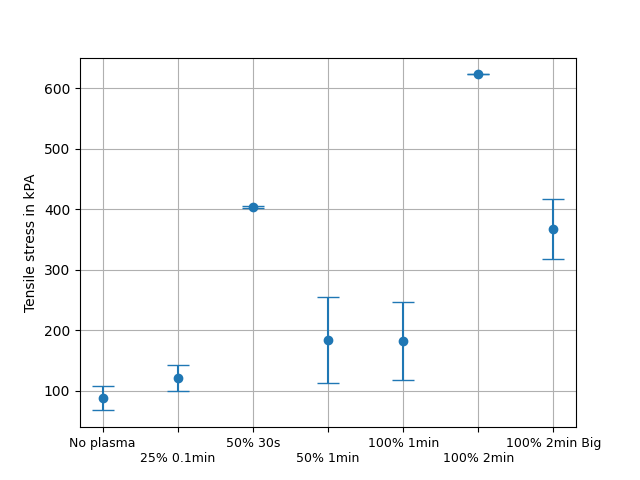
\includegraphics[width=14cm]{plot2_1PlasmaAktivierung}
\caption{PDMS 2:1 Vergleich bei verschiedenen Plasmacuring stärken und längen.}
\label{fig:PlotPlasmaAktivierung}
\end{figure}



